This example is presented to introduce \bioptim's ability to deal with a multiphase locomotion estimation problem including muscle actuation and contact forces.
The goal was to estimate muscle activations by tracking markers trajectories and ground reaction forces and moments. 
The model was a 3D leg with 12 DoFs (6-DoF pelvis, 3-DoF hip, 1-DoF knee and 2-DoF ankle), driven by 19 muscle activations and residual joint torques to compensate for potential muscle actuation weaknesses. 
The gait cycle was defined from the first heel strike to the end of the swing phase discretized into 90~shooting intervals. 
To approximate the natural rolling of the foot, the stance was divided into three phases (heel, flatfoot and forefoot contacts) of fixed duration deduced from experimental force platform data and markers position ($0.05$, $0.36$ and $\SI{0.16}{\second}$).
The swing phase lasted $\SI{0.38}{\second}$. 
The interaction between the ground and the foot was modeled using a four-contact points model located at the heel and the forefoot (first, fifth metatarsi and hallux).
The optimization problem consisted in minimizing the errors between predicted ($\bf{m}$) and reference ($\bf{m}^*$) markers trajectories, predicted ($\bm{\mathcal{F}}$, $\bm{\mathcal{M}}$) and reference ($\bm{\mathcal{F}^*}$, $\bm{\mathcal{M}}^*$) ground reaction forces and moments at all contact points.
A regularization term on muscle activations ($\bf{a}$) was also added (least-activations) as well as a penalization term on the residual torques ($\boldsymbol{\tau}$):

\[ 
\resizebox{0.9\columnwidth}{!}{$ 
\begin{aligned}
%\mathcal{J} = &\int_{t=0}^{T}\underbrace{\omega_1(\|m_p - m_m\|^{2})}_{\mathtt{TRACK\_MARKERS}}~ 
%+ ~ \underbrace{\omega_2(\|f_p - f_c\|^{2})}_{\mathtt{TRACK\_FORCES}}\\
%&+ ~ \underbrace{\omega_3(\|tau^f_p - tau^f_m\|^{2})}_{\mathtt{TRACK\_MOMENTS}}~
\mathcal{J} = &~\sum_{i=1}^4\left(\int_{T_{i-1}}^{T_i}\underbrace{\omega_1(\|\bm{m} - \bm{m}^*\|^{2})}_{\mathtt{TRACK\_MARKERS}}~ 
+ ~ \underbrace{\alpha\omega_2(\|\bm{\mathcal{F}} - \bm{\mathcal{F}}^*\|^{2})}_{\mathtt{TRACK\_FORCES}}\right.\\
&+ ~ \underbrace{\alpha\omega_3(\|\bm{\mathcal{M}} - \bm{\mathcal{M}}^*\|^{2})}_{\mathtt{TRACK\_MOMENTS}}~
+ ~ \underbrace{\omega_4\|\bf{a}\|^2}_{\mathtt{MIN\_ACTIVATION}}
+ ~ \underbrace{\|\boldsymbol{\tau}\|^2}_{\mathtt{MIN\_TORQUE}}~dt\left.\vphantom{\int_{T_{i-1}}^{T_i}}\right), 
\end{aligned}  
$}  
\addtag  
\label{eq:ocp_walk}  
\]

\begin{figure*}[t!] 
\centering 
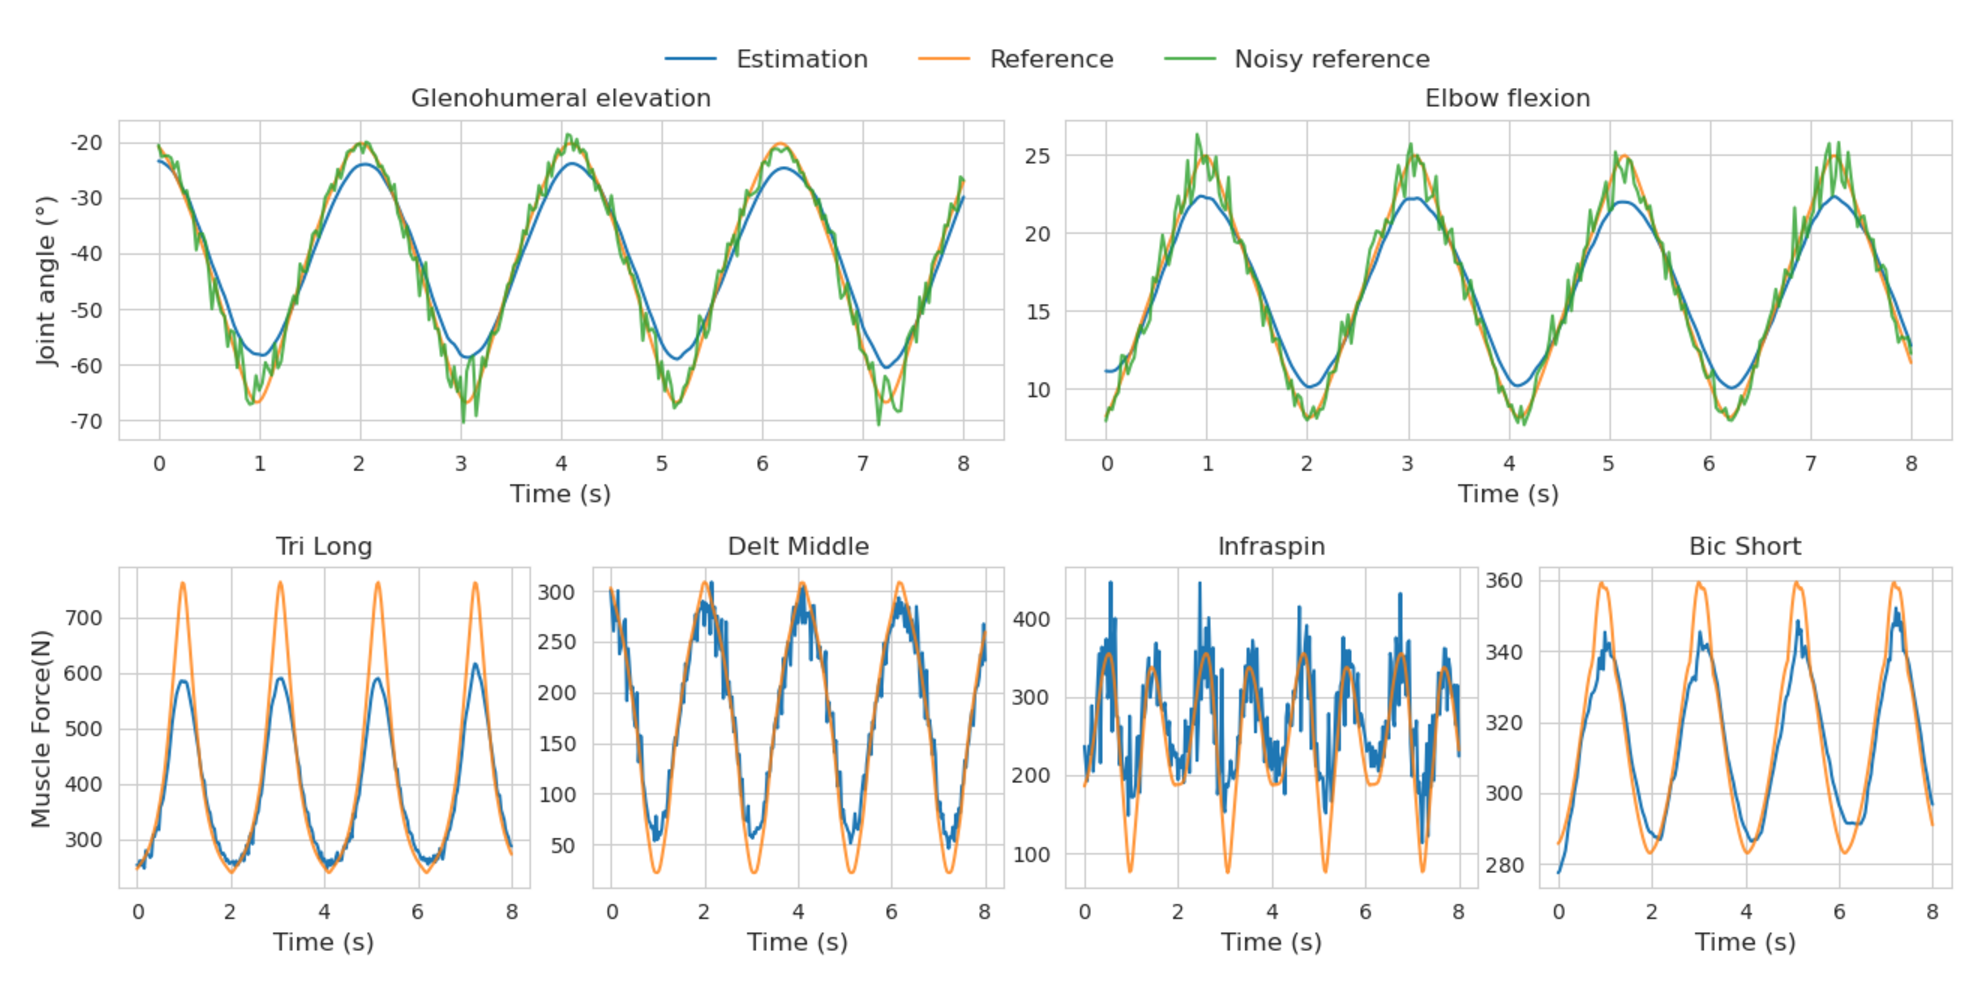
\includegraphics[width=\textwidth]{figures/MHE_results.pdf}\\
\caption{Ex.~\ref{ex:mhe}. Top row - Real-time estimated joint angles (blue), ground-truth joint angles (orange) and tracked noisy joint angles (green) for a cyclic motion of the arm.
Bottom row - Real-time estimated muscle forces (blue) and ground truth muscle forces (orange) for the same motion.
Only four muscles with significative action (peak forces $>$ $\SI{15}{\newton}$), on the two selected DoFs, are shown.
Muscle abbreviations stand for (from left to right): Triceps Long head, Deltoid Middle, Infraspinatus, Biceps Brachial Short head.} 
\label{fig:MHE_results}
\end{figure*} 
\noindent where $\omega_1=10^5$, $\omega_2=\omega_3=10^{-1}$, $\omega_4=10$ are weighting factors, $T_0=0$ and $T_i$, $i \in [1, 2, 3, 4]$, are the final time of the i$^{th}$ phase. 
Ground reaction forces and moments were only tracked during the stance phase, hence $\alpha = 0$ during the swing phase and $\alpha = 1$ otherwise. 
Non-slipping (\texttt{NON\_SLIPPING}) and unilateral contact force (\texttt{CONTACT\_FORCE}) constraints were added to prevent the foot from slipping and pulling from the ground. 
In between phases, the use of the \texttt{PhaseTransition.IMPACT} state transition allowed to represent the gain or loss of contact(s) in the dynamics (e.g., \cite{felis_synthesis_2016} swing phase to heel strike ).\\
Tracking experimental data allowed to reproduce leg motion during the walking cycle (Fig.~\ref{fig:snapshots_multiphase_walking_cycle}). 
The root mean square tracking error on markers trajectories was $\SI{27}{\milli\meter}$ (mean errors on pelvic and foot markers were $\SI{7.5}{\milli\meter}$ and $\SI{14.7}{\milli\meter}$, respectively). 
Concerning ground reaction forces tracking, the root mean square error was $\SI{27}{\newton}$.
During the stance phase, Gluteal muscles and Vastus Medialis were mainly activated during the loading response ($\SI{10}{\percent}$) and hamstrings during initial contact ($\SI{1}{\percent}$) (Fig.~\ref{fig:snapshots_multiphase_walking_cycle}). 
These results were similar to the characteristic average activity patterns of the lower limb muscles during locomotion described in~\cite{winter_biomechanics_1991}. 
The transition from stance to swing ($\SI{60}{\percent}$ - $\SI{70}{\percent}$) was highly actuated by hip flexors (Iliopsoas and Rectus Femoris) and leg muscles (Gastocnemius Medialis and Tibialis Anterior).

